\documentclass[0-protokol.tex]{subfiles}
\begin{document}
Osciloskop je jedním z nejčastěji používaných přístrojů ve fyzikální laboratoři. Umožňuje vizualizovat časový průběh napětí či s pomocí odporu zobrazit volt-ampérovou charakteristiku elektrické součástky. Zjednodušené schéma osciloskopu je zobrazeno na obrázku \ref{fig:osciloskop}.

\begin{figure}[H]
\centering
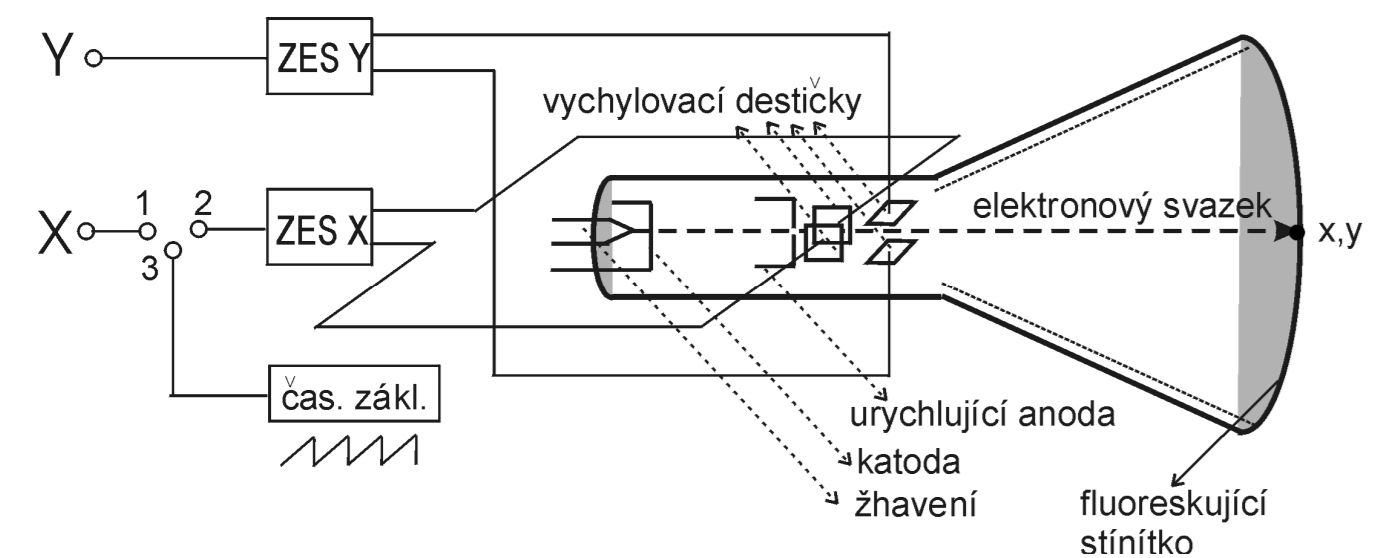
\includegraphics[scale=0.3]{osciloskop}
\caption{Zjednodušené schéma osciloskopu \cite{osciloskop}}
\label{fig:osciloskop}
\end{figure}

\subsection*{Střední, efektivní a špičková hodnota napětí}
Frekvence střídavého napětí je obvykle větší než doba kmitu systému analogového přístroje či doba jednoho
měření digitálního přístroje, tzv. integrační doba. Tyto přístroje proto nejsou schopné změřit \textit{okamžitou hodnotu} napětí $u(t)$, místo toho ukazují \textit{střední hodnotu} napětí, které se dá také vypočítat pomocí vztahu
\begin{equation}
U_e = \frac{1}{T} \int\limits_0^T u(t) dt,
\end{equation}
kde $T$ je perioda a $t$ čas.

\begin{figure}[H]
\centering
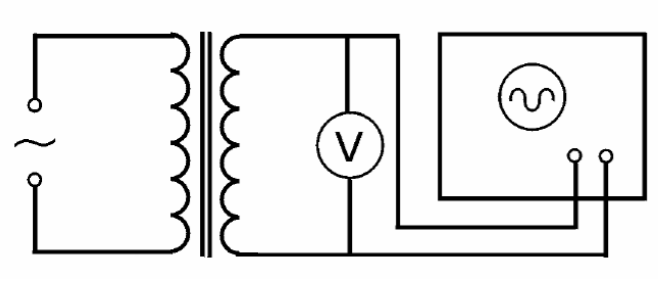
\includegraphics[scale=0.4]{zap_u1}
\caption{Zapojení pro měření špičkové hodnoty střídavého napětí}
\label{fig:zap_u1}
\end{figure}

Měřicí přístroje, určené k měření střídavého napětí sice měří střední hodnotu, jejich stupnice jsou však přepočítány na \textit{efektivní hodnotu} napětí, kterou lze spočítat pomocí
\begin{equation}
U^2 = \frac{1}{T} \int\limits_0^T u^2(t) dt.
\end{equation}
Je-li průběh napětí harmonický, platí 
\begin{equation} \label{eq:ef_napeti}
U = \frac{U_0}{\sqrt{2}},
\end{equation}
kde $U_0$ je \textit{špičková hodnota} - amplituda - napětí.

\subsection*{Jednocestný usměrňovač, filtrace napětí}
Jednocestný usměrňovač se používá k usměrnění střídavého napětí. Jeho zapojení s odporovou zátěží $R_Z$ je vyobrazeno na obrázku \ref{fig:jednocest_usm}. Průběh usměrněného napětí je zobrazen na obrázku \ref{fig:prubeh_jednocest}. Střední hodnotu takto usměrněného napětí lze spočítat podle vztahu
\begin{equation}
U_e = \frac{U_0}{\pi}.
\end{equation}

\begin{figure}[H]
\centering
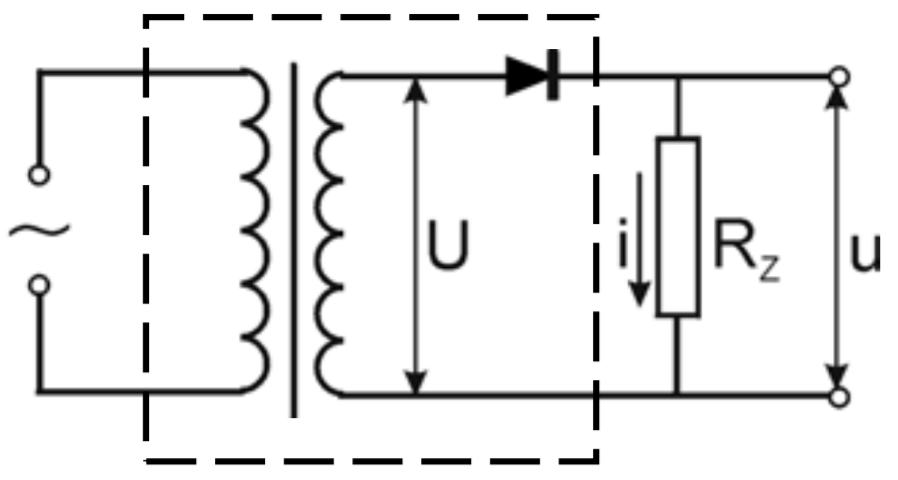
\includegraphics[scale=0.28]{jednocest_usm}
\caption{Schéma zapojení jednocestného usměrňovače s odporovou zátěží \cite{stud_text}}
\label{fig:jednocest_usm}
\end{figure}

\begin{figure}[H]
\centering
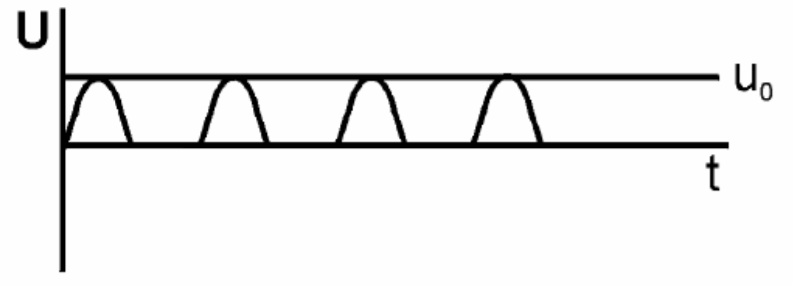
\includegraphics[scale=0.30]{prubeh_jednocest}
\caption{Průběh napětí usměrněného jednocestným usměrňovačem \cite{stud_text}}
\label{fig:prubeh_jednocest}
\end{figure}

Takto usměrněné napětí je pulzující, toto napětí můžeme vyhladit za pomoci kondenzátoru o kapacitě $C$ podle obrázku \ref{fig:zapojeni_filtrace}. Ten se periodicky nabíjí a následně vybíjí přes odpor $R_Z$ s časovou konstantou $\tau = R_Z C$. Aby se zabránilo přetížení zdroje při počátečním nabíjení kondenzátoru, je do obvodu zapojen ochranný odpor $R_{ochr.}$.

\begin{figure}[H]
\centering
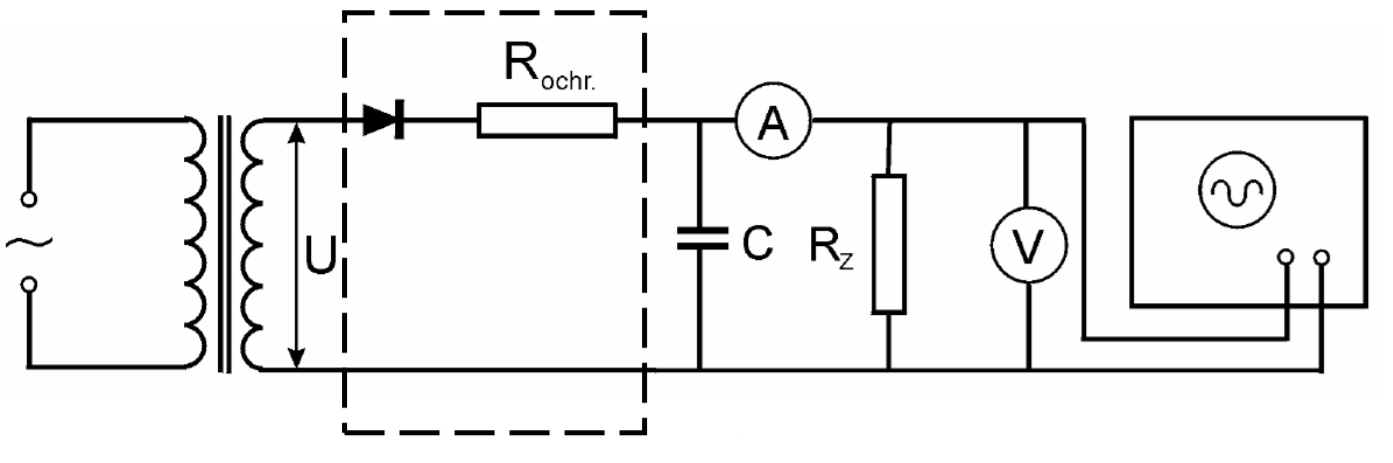
\includegraphics[scale=0.28]{zapojeni_filtrace}
\caption{Zapojení jednocestného usměrňovače s filtračním odporem, odporovou zátěží a měřicími přístroji \cite{stud_text}}
\label{fig:zapojeni_filtrace}
\end{figure}

Pro zjednodušení měření požadujeme, aby činitel filtrace $k_f$ byl velký. Činitel filtrace je definován jako
\begin{equation}
k_f = \frac{U_0}{\Delta U}
\end{equation}
a pro jednocestný usměrňovač platí
\begin{equation} \label{eq:cinitel_filtrace}
k_f = \frac{R_Z C}{T}.
\end{equation}
Odtud vyplývá, že abychom činitel filtrace udrželi konstantní, musíme s měnící se odporovou zátěží měnit i filtrační kapacitu $C$.

Proud zátěží $I_{SS}$ je s odporem $R_Z$ spojen Ohmovým zákonem
\begin{equation} \label{eq:ohmuv_zakon}
I_{SS} = \frac{U_{SS}}{R_Z},
\end{equation}
kde $U_{SS}$ je stejnosměrné napětí na zátěži. Pokud je $k_f$ výrazně větší než 1, je $U_{SS} = U_0$.

Podle \eqref{eq:cinitel_filtrace} a \eqref{eq:ohmuv_zakon} platí
\begin{equation}
C = \frac{T k_f I_{SS}}{U_0},
\end{equation}
tedy kapacita je přímo úměrná proudu.

\subsection*{Zobrazení V-A charakteristik}
Osciloskop umožňuje zobrazit průběh napětí jak na ose $X$, tak i $Y$. To znamená, že pomocí rezistoru známého odporu můžeme na ose $Y$ zobrazit proud, procházející součástkou, v závislosti na napětí. Pro toto měření použijeme zapojení z obrázku \ref{fig:volt-amper}.

\begin{figure}[H]
\centering
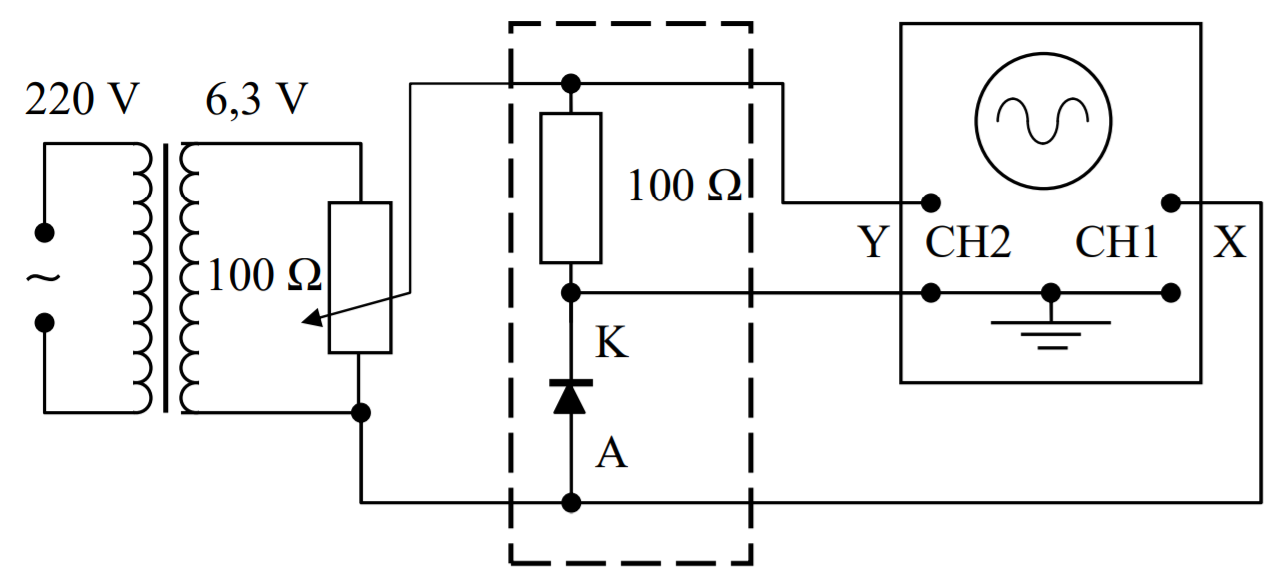
\includegraphics[scale=0.3]{volt-amper}
\caption{Zapojení použité pro zobrazení volt-ampérových charakteristik měřených součástek \cite{stud_text}}
\label{fig:volt-amper}
\end{figure}
\end{document}
